
\documentclass[submit]{ipsj}
%\documentclass{ipsj}
\usepackage[dvips]{graphicx}
\usepackage{latexsym}
\usepackage{pifont}


\def\Underline{\setbox0\hbox\bgroup\let\\\endUnderline}
\def\endUnderline{\vphantom{y}\egroup\smash{\underline{\box0}}\\}
\def\|{\verb|}

%%%%%%%%%%%%%%%%%%%%%%%%%%%%%%%%%%%%%%%%%%%%%%%%%%%%%%%%%%%%%%%%
%\bibliographystyle{ipsjsort}
%\usepackage{listings,jlisting}
\usepackage{listings}
\newcommand{\myvec}[1]{\vec{#1}}
\newcommand{\araa}{Annual Review of Astronomy and Astrophysics}
\newcommand{\icarus}{Icarus}
\newcommand{\mnras}{Monthly Notices of the Royal Astronomical Society}
\newcommand{\apj}{Astrophysical Journal}
\newcommand{\pasa}{Publications of the Astronomical Society of Australia}
\newcommand{\pasj}{Publications of the Astronomical Society of Japan}
\newcommand{\aap}{Astronomy and Astrophysics}
\newcommand{\nat}{Nature}
%%%%%%%%%%%%%%%%%%%%%%%%%%%%%%%%%%%%%%%%%%%%%%%%%%%%%%%%%%%%%%%%

\setcounter{巻数}{59}
\setcounter{号数}{1}
\setcounter{page}{1}


\受付{2016}{3}{4}
%\再受付{2015}{7}{16}   %省略可能
%\再再受付{2015}{7}{20} %省略可能
%\再再受付{2015}{11}{20} %省略可能
\採録{2016}{8}{1}




\begin{document}


\title{粒子法シミュレーションコード開発のためのフレームワーク(FDPS)の開発}

%\etitle{Development of Framework for Developing Particle Simulators (FDPS)}

%\affiliate{R-CCS}{理化学研究所計算科学研究センター\\
%IPSJ, Chiyoda, Tokyo 101--0062, Japan}


%\paffiliate{JU}{情報処理大学\\
%Johoshori University}

\affiliate{RIKEN}{理化学研究所 計算科学研究センター\\
7-1-26 Minatojima-minami-machi, Chuo-ku, Kobe, Hyogo,  650-0047, Japan}

\affiliate{KOBE}{神戸大学\\
1-1, Rokkodai-cho, Nada-ku, Kobe, 657-8501, Japan}

\affiliate{PEZY}{株式会社 PEZY Computing\\
1-11 Ogawa-machi, Chiyoda-ku, Tokyo,  101-0052, Japan}

\affiliate{EXA}{株式会社 ExaScaler\\
2-1 Ogawa-machi, Chiyoda-ku, 101-0052 Tokyo, Japan}

\author{岩澤 全規}{Masaki Iwasawa}{RIKEN}[masaki.iwasawa@riken.jp]
\author{行方 大輔}{Daisuke Namekata}{RIKEN}[daisuke.namekata@riken.jp]
\author{坂本 亮}{Ryo Sakamoto}{PEZY}[sakamoto@pezy.co.jp]
\author{中村孝史}{Takashi Nakamura}{PEZY}[nakamura@pezy.co.jp]
\author{木村耕行}{Yasuyuki Kimura}{EXA}[yasuyuki@exascaler.co.jp]
\author{似鳥啓吾}{Keigo Nitarori}{RIKEN}[keigo@riken.jp]
\author{野村昴太郎}{Kentaro Nomura}{RIKEN}[kentaro.nomura@riken.jp]
\author{坪内美幸}{Miyuki Tsubouchi}{RIKEN}[miyuki.tsubouchi@riken.jp]
\author{牧野 淳一郎}{Junichiro Makino}{KOBE, RIKEN}[jmakino@riken.jp]

\begin{abstract}

粒子法は粗密の大きい系や空隙のある系のシミュレーションに強く,科学や工
学の幅広い分野で使われている.しかし、「京」の様な大規模並列計算機で効
率よく動作する並列シミュレーションコードを開発することは容易ではなく,
多くの研究者がコードの開発に膨大な時間を割いているのが現状である.しか
し、粒子法シミュレーションコードの効率の良い並列化のアルゴリズムは,シ
ミュレーション対象によらず似ている.そこで,我々は粒子法コードの開発を
容易にするためのフレームワークFDPS(Framework for Developing Particle
Simulators)の開発を行った.我々はC++のテンプレート機能を用いてFDPSを開
発した.これは,ユーザーが定義する粒子のデータ構造と相互作用を扱えるよ
うにするためである.我々の経験では,FDPSを使うことで様々なアプリケーショ
ンが数百行で書ける.また相互作用カーネルを十分最適化すれば開発したアプ
リケーションは多くのスパコン上で理論ピーク性能の30-50\%程度の実行効率
で動作する.\\

本稿ではFDPSの概要および,Ver.1リリース後に追加された新機能,特にアク
セラレータを持つ計算機を効率よく使うためのマルチウォーク法や相互作用リ
ストを再利用する機能,さらにFDPSをC++言語以外から使うための多言語イン
ターフェースについて報告する.

\end{abstract}


\begin{jkeyword}
HPC,フレームワーク,粒子法
\end{jkeyword}

\maketitle

%1
\section{はじめに}

粒子法とは研究対象となる系を多数の相互作用を及ぼしあう粒子の集団として
表現し,その発展方程式を解くことで,系の進化を追跡する手法である.粒子
は発展方程式に従い自動的に移動するため,粗密の大きな系や空隙のある系,
また物体の衝突や破壊などのシミュレーションに強く,自然科学や工学の様々
な分野で用いられている.近年,スーパーコンピュータは大規模並列化がすす
み,より大規模,高解像度のシミュレーションを行うためには粒子法シミュレー
ションコードの効率の良い並列化が必須となってきた.

効率の良い並列粒子法コードを開発するためにはアプリケーションプログラマー
はロードバランスを考慮したシミュレーション領域の動的分割を考える必要が
ある.また,計算領域が分割されているので,各プロセスは相互作用計算を行
うために他プロセスの持つ粒子の情報を必要とするが,この時の他プロセスと
の通信量を小さくする必要もある.アプリケーションプログラマーは上記のよ
うな事柄を考慮してシミュレーションプログラムを開発する必要があるが,こ
れらを考慮してアプリケーションプログラムを開発することは容易ではなく,
多くの研究者がプログラム開発に膨大な時間を割いているのが現状である.

並列化された粒子法シミュレーションプログラムは数多く存在する
\cite{1995LAMMPS}\cite{2005MNRAS.364.1105S}\cite{2009PASJ...61.1319I}\cite{2014GROMACS}\cite{Bedorf:2014:PGT:2683593.2683600}
が,それらの多くはシミュレーションする対象が限定されており,他の分野へ
それらのコードを適用する事は難しい.また,数値計算スキームも固定されて
いるため,新しいアルゴリズムを開発したとしても,それらのプログラム上で
新しいアルゴリズムを用いる事は困難である.

しかし,シミュレーションする対象が違っても効率の良い並列化アルゴリズム
は大きくは変わらない.そこで,我々は並列粒子法コードの開発を容易にする
ためのフレームワークFDPS(Framework for Developing Particle Simulators)
の開発を行い,2015年3月にFDPSver.1のリリースを行った
\cite{2016PASJ...68...54I}.FDPSは並列粒子シミュレーションコードのため
に必要な関数を備えたC++のテンプレートライブラリであり,アプリケーショ
ンプログラマは行いたいシミュレーションに合わせて粒子データと相互作用関
数を定義し,FDPSのAPIを用いて容易にプログラム開発する事ができる。実際,
我々はFDPSを用いて,N体シミュレーションやSPHシミュレーションコードを容
易に開発できることを確認した.さらに,「京」等の大規模並列計算機上でシ
ミュレーションを行い,アプリケーションの性能を測定した.FDPSを使って書
かれたアプリケーションの実行効率は30-50\%と非常に高い事も確認した.

本稿ではVer.1リリース後,現在(2018年11月)の最新バージョンであるVer.5ま
でに追加した機能について,特にアクセラレータを持つ計算機を効率よく使う
ためのマルチウォーク法や相互作用リストを再利用する機能,さらにFDPSを
C++言語以外から使うための多言語インターフェースについて報告する
\cite{2018PASJ...70...70N}.本稿の構成は以下のとおりである.2節では
FDPSの概要について述べる.3節ではVer.2およびVer.4で追加されたアクセラ
レータ向けの新機能について述べる.4節ではVer.3およびVer.5で追加された
C++以外の言語からFDPSを使用するための多言語インターフェースについて述
べる.5節で本稿をまとめる.

%2
\section{FDPSの概要}

\subsection{FDPSのデザインコンセプト}

FDPS開発の基本的なアイディア(そして、最終的なゴール)はアプリケーショ
ンプログラマーが効率の良い並列粒子シミュレーションコードを短時間で開発
できるようにする事である.そのためにFDPSは効率の良いプログラムを開発す
るために必要なAPIを持っている.これらのAPIから呼び出されるFDPS内部の関
数はMPIおよびOpenMPにより並列化がされているためにユーザーは特に並列化
を意識することなく並列化粒子シミュレーションコードを開発することができ
る.また,FDPSは任意の粒子間相互作用を扱えるようにC++のテンプレート機
能を用いて開発されている。アプリケーションプログラマは粒子のデータ構造
と相互作用関数を定義し,さらにFDPSが提供しているAPIを用いてプログラム
開発を行う事が要求される.

\subsection{FDPSを用いた粒子シミュレーションの流れ}

FDPSを用いた粒子シミュレーションの流れは以下のとおりである.
\begin{enumerate}
\item 各プロセスから粒子をサンプルし,サンプルした粒子からマルチセクショ
  ン法\cite{2004PASJ...56..521M}により計算領域の分割を行う.
\item 各プロセスが担当する粒子が担当する領域内に収まるように,プロセス
  間で粒子の交換を行う.
\item 各プロセスが担当する粒子のみで木構造(ローカルツリー)を構築する.
\item 各プロセスが他のプロセスが相互作用計算を行うために必要な情報
  (LET:Local Essentail Tree)を他の全てのプロセスへ送る.
\item 担当している粒子とLETを用いて木構造(グローバルツリー)を再び構築.
\item 木構造を用いて相互作用リストを作成し相互作用を計算.
\item 相互作用計算の結果を用いて粒子の物理量を更新する.
\item 1に戻る.
\end{enumerate}

上記の手順1から6までをFDPSは担当する.手順1,2,3--6に対応して,FDPSは
{\tt DomainInfo},{\tt ParticleSystem},{\tt TreeForForce}と呼ばれる
C++のクラスを持ち,ユーザーはこれらのクラスのメンバ関数を用いてプログ
ラム開発を行う.そのため,初期のFDPSではアプリケーションプログラムを
C++で書く必要があった.しかし,最新バージョンであるVer.5ではFORTRANやC
言語からもFDPSを使用するためのインターフェースが導入されている.これに
ついては\ref{sec:if}節で詳しく述べる.

\subsection{FDPSの開発史}

FDPSは2015年3月のリリース以降,2018年11月までに4回のメジャーアップデー
トを行ってきた.FDPSのメジャーアップデートの歴史とその時の主な機能追加
は以下のようになっている.

\begin{itemize}
\item 2015年3月 Ver.1をリリース.
\item 2016年1月 Ver.2をリリース.マルチウォーク法を導入.
\item 2016年12月 Ver.3をリリース.Fortranインターフェースを追加.
\item 2017年11月 Ver.4をリリース.相互作用リストを再利用する機能を導入.
\item 2018年11月 Ver.5をリリース.C言語インターフェースを追加.
\end{itemize}

Ver.1では主に「京」のような汎用CPUをベースとした大規模並列計算機で性能
が出るように開発された.しかし,ここ10年ほどでGPGPU(General Purpose
Graphics Processing Units)等のアクセラレータを搭載したスパコンが増えて
きており,FDPSもそれらの計算機に対応させる必要があった.そこで、Ver.2
からは浜田等\cite{Hamada:2009:THN:1654059.1654123}によって開発されたマ
ルチウォーク法をFDPSに導入しアクセラレータ対応を図った.さらにVer.4か
らは,同じツリー構造や相互作用リストを複数ステップの間使い続ける機能を
導入した.さらに,ホストとアクセラレータ間での相互作用リストの転送量を
減らすために,相互作用計算を始める前に全粒子とLETをアクセラレータに送
り,相互作用リストとしては粒子のアクセラレータ上でのアドレスのみを送る
方法も導入した.Ver.2およびVer.4で追加されたこれらの機能については
\ref{sec:acc}節で詳しく解説する.

FDPSはC++により開発されており,Ver.1ではアプリケーションプログラマは
C++言語によりアプリケーションを書くことが求められていた.しかし,HPCで
はFORTRANやC言語もよく用いられており,C++になじみの薄い開発者も多い.
そこでVer.3ではFDPSをFortranから呼び出すためのインターフェースの開発を
行った.またVer.5では同様にC言語からもFDPSを呼び出すことのできるインター
フェースの開発を行った.Ver.3およびVer.5で追加されたこれらのインター
フェースについては\ref{sec:if}節で詳しく解説する.

\section{アクセラレータ対応}
\label{sec:acc}

本節ではGPGPU等のアクセラレータを持つ計算機上で高い実行効率を達成する
ために追加された機能について述べるo.追加された機能は大きく以下の3つで
ある.

\begin{itemize}
\item マルチウォーク法
\item 粒子への間接アドレス指定 
\item 相互作用リストの再利用
\end{itemize}

以下これらの機能について解説する.

\subsection{マルチウォーク法}

FDPSでは相互作用関数をユーザーが任意に定義できるため,粒子法で最もコス
トがかかる相互作用計算のみをアクセラレータで行わせることができる。しか
し,Ver.1ではアクセラレータを持つ計算機では高い実行効率をあげる事は困
難であった.これは以下の理由による.FDPSでは相互作用の計算にはBarnesに
よって開発された手法\cite{1990JCoPh..87..161B}を用いている.これは一つ
の粒子に対して相互作用リストを作るのではなく,近傍にいる粒子をグループ
化し,その粒子グループについて相互作用リストを作り,相互作用を計算する
手法である.Ver.1では一つの粒子グループに対して相互作用リストをつくり
計算するということを繰り返し行っていた.しかし,GPGPU等のアクセラレー
タではカーネルの起動オーバーヘッドが大きく相互作用リストの数が大きくな
るとこのオーバーヘッドが無視できなくなる.また,非常に大量の演算コアを
搭載しているため,1つの相互作用リストについて計算するだけでは全ての演
算コアを使いきることはできない.そこで,Ver.2ではマルチウォーク法と呼
ばれる手法を導入した.

マルチウォーク法では、FDPSは一度に複数の相互作用リストを作り,それらを
まとめてアクセラレータに転送し相互作用計算を実行する.これにより、カー
ネル起動オーバーヘッドを削減でき,また全ての演算コアを動作させることが
できる.さらに,アクセラレータでの相互作用計算を行っている間にCPU側で
次の相互作用リストを作ることができるため,相互作用リスト作成にかかる時
間を隠ぺいすることができる.

\subsection{粒子への間接アドレス指定}
\label{sec:adr}
アクセラレータを搭載している計算機上で相互作用リストを用いて計算を行う
簡単な方法の一つは,それぞれの粒子グループとそれに対応する相互作用リス
トに対して,計算に必要な物理量をアクセラレータに送り計算する事である.
しかし,相互作用リスト内の粒子数は非常に大きく,大雑把にはローカルに存
在する粒子数の10倍以上になる.一般に,LETの数はローカルの粒子数より非
常に少ないので,これは同じ粒子をアクセラレータに10回以上送っている事を
意味する.

同じ粒子を複数回送らないようにするためには,相互作用計算を始める前に全
てのローカル粒子とLETをアクセラレータに送ってしまい,相互作用リストに
は粒子もしくはLETのアクセラレータ上でのインデックスのみを記憶させれば
よい.こうすることで相互作用の時に粒子の物理量を送るのではなく,インデッ
クスだけを送ればよいことになる.これにより,例えば重力計算の場合は粒子
のデータサイズが16バイト程度であるのに対して,インデックスは4バイトあ
ればよいので転送データサイズを四分の一にできる.また,SPH等の流体シミュ
レーションの場合は粒子データが50バイト程度になることもあり,転送量を十
分の一にすることができる.

\subsection{相互作用リストの再利用}

SPHシミュレーション等の流体計算や分子動力学シミュレーション等では安定
性条件から時間刻みが制限されるため,粒子が時間刻みあたりに移動する距離
は短い.そのため,一度作った相互作用リストを複数時間刻みの間,再利用す
ることができる.また,重力N体シミュレーションの場合でも,例えば惑星形
成シミュレーションや惑星系リングのシミュレーションなどでは,時間刻み当
たりの粒子間距離の変化は小さく,相互作用リストの再利用が可能である.銀
河形成シミュレーション等のN体+SPHシミュレーションの場合等でも,時間刻
みは流体粒子の時間刻みできまり,この刻みの間ではN体粒子の移動距離は短
いと考えられるためやはり,相互作用リストの再利用は可能である。このため,
FDPS Ver.4では相互作用リストの再利用を行う機能を搭載した.

相互作用リストを再利用した場合には相互作用リストを構築するステップ
(construction step)とリストを再利用するステップ(reuse step)の手順は異
なる.construction step時相互作用計算の手順は以下のとおりである.

\begin{enumerate}
\item ローカルツリーを構築する.
\item LETを交換する.
\item グローバルツリーを構築.
\item 木構造を用いて相互作用リストを作り、相互作用を計算。この時相互作
  用リストを記憶する.
\item 相互作用計算の結果を用いて粒子の物理量を更新する.
\end{enumerate}

construction step時の手順に対して,reuse step時の手順は以下のようにな
る.
\begin{enumerate}
\item ローカルツリーの物理量を更新する.
\item LETを交換する.
\item グローバルツリーの物理量を更新する.
\item 記憶されている相互作用リストを用いて相互作用を計算.
\item 相互作用計算の結果を用いて粒子の物理量を更新する.
\end{enumerate}

つまり,reuse stepでは以下の手順を省くことができる.a)木構造の構築,
b)LETの構築,c)相互作用リストの構築.a)の計算コストはO($n$)であり,b)
およびc)の計算コストはO($n$log$n$)となる.それゆえ,これらの計算時間は
無視できるものではなく,これらの手順を省ける事による効果は大きい.

\subsection{API}

この節では3.1から3.3節で述べた機能を使用するためのAPIについて述べる.

FDPSでは一回のAPI呼び出しで,相互作用計算に必要な計算を全て行う高レベ
ルAPIが存在する.マルチウォーク法を用いる場合は,ユーザーは{\tt
  CalcForceAllAndWriteBackMultiWalk}もしくは{\tt
  CalcForceAllAndWriteBackMultiWalkIndex}を使用すればよい.これら二つ
の関数の違いは\ref{sec:adr}節で述べた粒子への間接アドレス指定を用いる
かどうかである.どちらの関数を使用する場合でもリストを再利用することは
可能である.リストを再利用するかどうかは上記の高レベル関数の引数として
指定する.

図\ref{code:main}はメイン関数の例である.6,7,8行目で{\tt
  ParticleSystem}クラス,{\tt DomainInfo}クラス,{\tt TreeForForce}ク
ラスのオブジェクトを生成している.14行目からが時間積分のループである.
この例では8ステップごとに領域分割(17行目),粒子交換(18行目),ツリーと
相互作用リスト作成を行っている.{\tt
  CalcForceAllAndWriteBackMultiWalkIndex}の最後の引数に{\tt
  MAKE\_LIST\_FOR\_REUSE}を用いることで,FDPSは木構造や相互作用リスト
を作成し,それらを内部に保存する(construction step).reuse stepでは引
数に{\tt REUSE\_LIST}を与えることで,FDPSは内部に保存されているツリー
や相互作用リストを使用し,相互作用計算を行う.

マルチウォーク法を使用する場合はユーザー定義の相互作用関数は2つの部分
に分ける必要がある.一つはdispatch関数(22行目)と呼ばれるもので,ホスト
からアクセラレータへの転送および,アクセラレータ上で実行される相互作用
計算のためのカーネルを起動させるためのものある.もう一つはretrieve関数
(23行目)と呼ばれアクセラレータ内での計算結果を回収するためのものである.

関数が二つに分かれている理由はアクセラレータで相互作用を計算している間
に次の粒子グループの相互作用リストを作り,また既に相互作用を計算した粒
子の積分を行うことで,これらにかかる時間を隠ぺいするためである.

dispatch関数およびretrieve関数の実装例についてはFDPS付属のサンプルコー
ドを参照されたい.

\begin{figure}[!h]
\begin{lstlisting}[language=c++,numbers=left,numbersep=5pt,frame=single,basicstyle=\ttfamily]
using namespace PS:    
int main(int argc, char *argv[]) {
      
  // FDPSの初期化(省略)
  
  ParticleSystem<FP> system;
  DomainInfo dinfo;
  TreeForForceLong<FORCE,EPI,EPJ>::Monopole
    tree;

  // 初期条件設定(省略)

  int n_loop =0;
  while(time_sys < time_end){
    INTERACTION_LIST_MODE int_mode=REUSE_LIST;    
    if(n_loop % 8 == 0){
      dinfo.decomposeDomainAll(system);
      system.exchangeParticle(dinfo);
      int_mode = MAKE_LIST_FOR_REUSE;
    }
    tree.calcForceAllAndWriteBackMultiWalkIndex
      (DispatchKernelIndex,
       RetrieveKernel,
       tag_max,
       system,
       dinfo,
       n_walk_limit,
       true,
       int_mode);

    // 軌道積分(省略)

    n_loop++;
  }
  return 0;
}

\end{lstlisting}
\caption{メイン関数の例.この例では,8ステップ毎にツリーと相互作用リス
  トを作り直している.}
\label{code:main}
\end{figure}
  
\subsection{性能}

この節では,上記の三つのアルゴリズムを用いた場合のN体シミュレーション
コードの性能について述べる.\ref{sec:single_node}節ではCPUのみを用いた
場合とアクセラレータとしてGPGPUを用いた場合のシングルノードでの性能を,
\ref{sec:multiple_node}節ではヘテロジニアスメニーコアであるSunway
26010とPEZY-SC2を用いた大規模並列システムでの性能について述べる.

\subsubsection{GPGPUを用いた場合のシングルノードでの性能}
\label{sec:single_node}

アクセラレータとしてNvidia TITAN Vを用い,ホストCPUはIntel Xeon
E5-2670 v3を用いた.これらの演算性能は単精度の場合13.8Tflops,883Gflops
である.ホストのメインメモリはDDR4であり,理論ピーク転送速度は68 GB/s.
CPUとGPGPUはPCI Express 3.0で接続されており,理論ピーク転送速度は15.75
GB/sである.

シミュレーションの初期条件としては速度分散がない一様球を考える.この場
合,系は自己相似的に崩壊するため,相互作用リストの再利用が可能である.
粒子数は4M(=$2^{22}$)とし、ツリーのオープニングクライテリオン$\theta$
は0.5とした.

図~\ref{fig:wtime_ngrp_th0.5}はCPUを使用した場合とGPGPUを使用し上記の
三つのアルゴリズムを用いた場合の時間ステップ当たりの計算時間を表してい
る.横軸は相互作用リストを共有する粒子の数の平均である(平均i粒子数)。
計算時間は平均i粒子数に依存するが、最適な平均i粒子数では、CPUのみを用
いた場合に対して,GPUを用いた計算はconstruction stepで3倍,reusing
stepで10倍ほど速くなっていることが分かる.つまり,GPUを用いVer.5までに
追加された機能を用いることで,CPUを用いVer.1の機能のみを使った場合に比
べて最大で10倍高速に計算する事が可能になった.

また,最適な平均i粒子数での計算速度はCPUのみを用いた場合は432Gflopsで
ありこれは理論ピーク性能の49\%にあたる.GPUを用いた場合の計算速度は
construction stepで3.0Tflops,reuse stepで4.5Tflopsであり、これはそれ
ぞれ、理論ピーク性能の22\%と33\%にあたり、非常に高い効率で動作している
ことが分かる.


\begin{figure}[!h]
    \begin{center}
      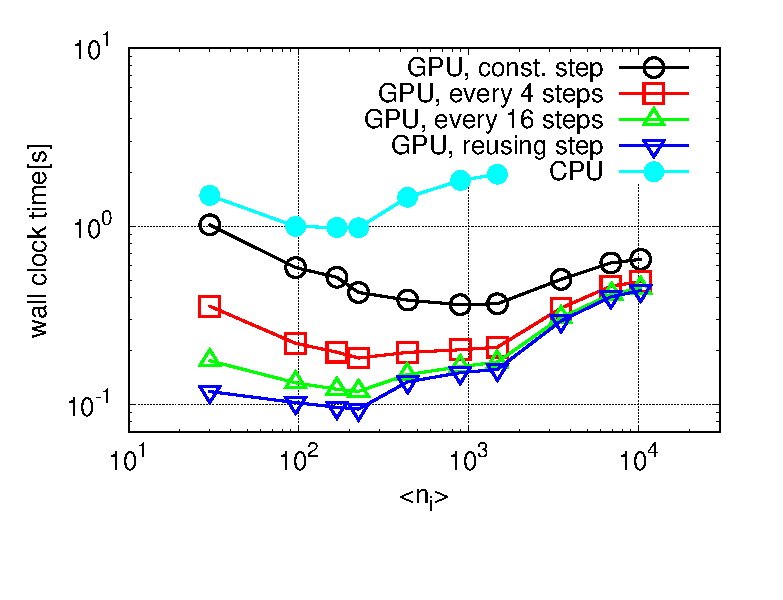
\includegraphics[width=8cm]{./fig/wtime_ngrp_th0.5.eps}
    \end{center}
    \caption{ステップ当たりの計算時間を平均i粒子数に対してプロットした.}
  \label{fig:wtime_ngrp_th0.5}
\end{figure}


\subsubsection{大規模並列ヘテロジニアスメニコアシステムでの性能}
\label{sec:multiple_node}

ここでは大規模並列システムでの性能について述べる.ここでは計算機として
以下の3システムを使用した.

\begin{itemize}
\item Taihulight
\item Gyoukou
\item Shoubu System-B
\end{itemize}

Taihulightは40960個のSunway 26010プロセッサからなる
\cite{{fu2016sunway}}.1つのSunway 26010プロセッサは4つのCore
Group(CG)からなり,1つのCGには1個のMPE(Management Processing Element)
と64個のCPE(Computing Processing Element)からなる.各CGはDDR3のメイン
メモリをもち,理論ピーク転送速度は34 GB/sである.各PEのクロックは1.45
GHzであり,1サイクルに4つの倍精度FMAを行う事ができるため,CG当たりの理
論ピーク性能は754Gflopsである.我々はTaihuLightをもちいるときは1つのCG
に1つのMPIプロセスを割り当てた.

GyoukouおよびShoubu System-Bはそれぞれ13312個と512個のPEZY-SC2プロセッ
サチップからなる.各チップはDDR4のメインメモリをもち,理論ピーク転送速
度は76.8GB/sである.PEZY-SC2プロセッサは2048個のコア(有効なコアは1984
個)からなる.各コアは1サイクルに倍精度の積和演算を一回実行することがで
きる.単精度や半精度の場合は2もしくは4ウェイのSIMDとして動作し,コアの
動作周波数は700MHzである.そのため,1チップあたりの理論ピーク性能は倍
精度で2.8Tflops,単精度で5.6Tflops,半精度で11.1Tflopsとなる.我々は
PEZY-SC2ベースのシステムを使用するときは一つのチップに一つのMPIプロセ
スを割り当てた.また,相互作用の計算には単精度を使用した.

これらのシステムを用いて我々は土星の環のシミュレーションを行った.粒子
数はMPIプロセスあたりに$10^7$個とした.図\ref{fig:perf}は弱スケーリン
グでの性能である.全てのシステムで非常によくスケールしていることが分か
る.性能はShoubu System-Bの512プロセスで1.01Pflops,Gyoukouの8192プロ
セスで10.6Pflops,TaihuLightの16万プロセスで47.9Pflopsである.これはそ
れぞれ理論ピーク性能の35.5\%,23.5\%,40.0\%にあたる。同じPEZY-SC2のシ
ステムであるが,Gyoukouの性能がShoubu System-Bの性能よりも低いのは
Gyoukouが2018年3月に停止したため,コードのチューニングが十分でなかった
ためである.なお、これらの計算に使用したコードでは大規模リング計算向け
の最適化も行われている.詳細は\cite{2018ICCS}にある.

\begin{figure}[!h]
    \begin{center}
      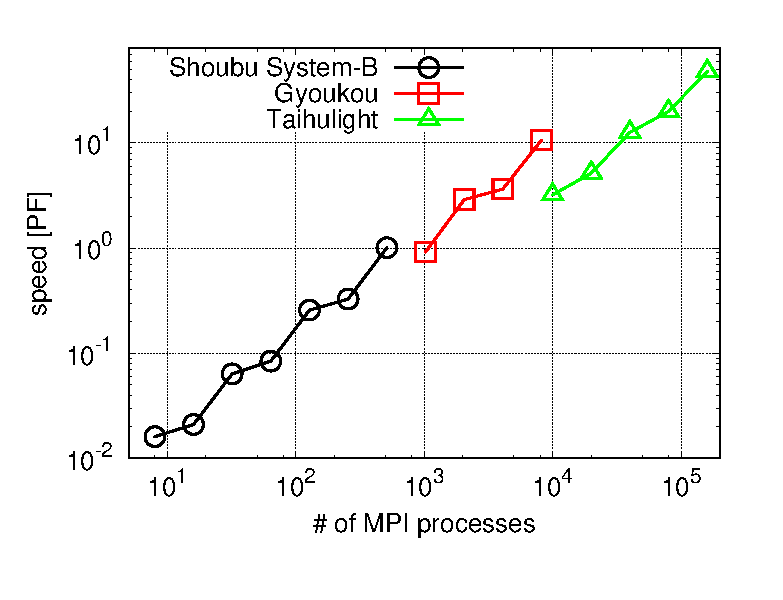
\includegraphics[width=8cm]{./fig/perf.eps}
    \end{center}
    \caption{弱スケーリング時の性能.縦軸はPetaFlops単位での計算速度、
      横軸はMPIのプロセス数.}
  \label{fig:perf}
\end{figure}


\section{多言語インターフェース}
\label{sec:if}

\subsection{インターフェースの設計}
Fortran/C言語インターフェースを開発する上での一つの困難は,FortranやC言語からC++のテンプレート機能を直接利用する手段がないことである.二節で述べた通り,C++のテンプレート機能はFDPSに任意の粒子データ型や粒子間相互作用をサポートさせる上で不可欠なものであった.したがって,Fortran/C言語インターフェースでも任意の粒子データ型や粒子間相互作用をサポートするためには,何らかの方法でこの問題を解決する必要がある.

我々は以下の事柄を組み合わせてこの問題を解決した.(i) C++関数は\texttt{extern "C"}修飾子によってC言語からも呼び出せる事,(ii) FDPSのC++コア部(C++で実装されたFDPSの部分)を操作するC++プログラムの自動生成,(iii) Fortran 2003で導入されたFortranとC言語の相互運用を保証する仕組み.(i)と(iii)によって,\textsl{特定の}粒子データ型向けに作られたFDPSライブラリ(C++コア部を操作する一連のC++関数群のことと定義)をFortranやC言語から利用可能になる.しかしながら,実現したいのは\textsl{任意の}粒子データ型を扱えるFDPSライブラリをFortranやC言語から利用できるようにすることである.これを実現する唯一の方法は,与えられた粒子データ型に応じたFDPSライブラリを生成することである.我々はFDPSの利用者がFortanやC言語のみで,アプリケーションを開発できるようにしたいので,それぞれの言語で粒子を表すデータ構造からFDPSライブラリを生成する必要がある.我々は粒子を表すためのデータ構造として,Fortranでは派生データ型,C言語では構造体を採用した.したがって,我々の解決案は次のようなものである.まず,FDPSの利用者は Fortran 2003の派生データ型 或いは C言語の構造体で粒子を定義する.次に,この粒子データ型に対応するC++クラスを生成する.最後に,このC++クラス向けのFDPSライブラリを生成する.これが(ii)が必要な理由である.これらの生成は我々が用意する\textsc{Python}スクリプトが自動的に行う.

残る問題点は,どのようにしてFortran 或いは C言語で書かれた粒子データ型から対応するC++クラスを生成するのかということである.適切な生成には,以下の情報が必要となる.
\begin{itemize}
\item データ型が粒子を表すものであること.
\item データ型のどのメンバ変数がFDPSが必要とする物理量に対応するか.FDPSは粒子の位置等,特定の物理量を必要とする.C++からFDPSを利用する場合,利用者に位置を返すメンバ関数等,いくつかのメンバ関数を定義してもらうことでこの問題を解決する設計となっていた.しかしながら,Fortranの派生データ型やC言語の構造体はメンバ関数は持てない.
\end{itemize}
我々は独自の指示文を導入してこの問題を解決した.指示文は特定のフォーマットのコメント文で,自動生成を行う\textsc{Python}スクリプトに必要な情報を渡すために使用される.具体的には,例えばFortranの場合,派生データ型名の隣にコメント文\texttt{!\$fdps FP}を記述すると,スクリプトは,この派生データ型がFullParticle型であると解釈する.ここで,FullParticle型は粒子のすべての情報を持つデータ型のことである.同様に,メンバ変数名の隣にコメント文\texttt{!\$fdps position}を記述すると,このメンバ変数は粒子の位置を表すとスクリプトは解釈する.このような指示文を用いることで,スクリプトは必要なC++クラスを生成することが可能となる.

以上がFortran/C言語インターフェースの設計である.図\ref{fig:if_design}は,インターフェースの仕組みを模式的に表したものである.まずユーザは粒子をFortranの派生データ型 或いは C言語の構造体で定義する.このとき,指示文を使って必要な情報も記述する(ステップ\ding{192}).自動生成スクリプトは,ユーザが書いたソースコードの中から指示文を手がかりに粒子を表す派生データ型 ないしは 構造体を自動的にすべて見つけ,対応するC++クラスを(複数)生成する(ステップ\ding{193}).同時に,これらC++クラス向けのFDPSライブラリを生成する(ステップ\ding{194}).これはC++から利用可能なFDPSのAPIとほぼ同じものを提供するC++関数群から構成される.スクリプトはこのC++関数群のC言語インターフェースも生成する(ステップ\ding{195}).これがFDPSのC言語インターフェースと呼んでいるものである.Fortranから使用可能にするためのFortranモジュールも生成される(ステップ\ding{196}).このモジュールはFortran用のインターフェースを提供する.ユーザはこれらのインターフェースで提供されるAPIを使用して,アプリケーションを開発する(ステップ\ding{197}, \ding{197}').
\begin{figure}
\centering
\includegraphics[width=8cm]{./fig/if_design.eps}
\caption{Fortran/C言語インターフェースの仕組み}
\label{fig:if_design}
\end{figure}

\subsection{インターフェースの利用例}
本節ではC言語インターフェースの利用例を簡単に説明する.前節で述べた通り,ユーザはまずC言語の構造体と指示文を用いて粒子を定義する必要がある.そこで,粒子を定義したC言語ソースファイルの例を図\ref{fig:src_fp_in_c}に示す.
\begin{figure}
\centering
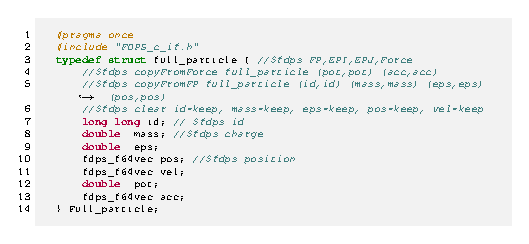
\includegraphics[width=8cm]{./fig/src_fp_in_c.eps}
\caption{C言語での粒子の実装例}
\label{fig:src_fp_in_c}
\end{figure}
上から順に説明していく.まず,ファイル冒頭でヘッダーファイル\texttt{FDPS\_c\_if.h}がインクルードされている.このヘッダーファイルにはFDPSのC言語用APIのプロトタイプ宣言やFDPSから提供されるデータ型が記述されており,これらを使用する場合には必ずインクルードする必要がある.

次に構造体タグ名の右隣に以下のコメント文がある.
\begin{lstlisting}
//$fdps FP,EPI,EPJ,Force
\end{lstlisting}
これはこの構造体が粒子であることを示す指示文である.文字列\texttt{//\$fdps}で始まるコメント文はすべて自動生成スクリプトに指示文として解釈される.文字列\texttt{//\$fdps}の右側には粒子の種別を表すキーワードが続いる.\texttt{FP}はFullParticle型,\texttt{EPI}はEssentialParticleI型,\texttt{EPJ}はEssentialParticleJ型,\texttt{Force}はForce型であることを示すキーワードである.複数のキーワードが指定された場合,それらを同時に兼ねることを示す.FullParticle型以外のデータ型の定義についてはFDPSの仕様書を参照されたい.

メンバ変数宣言部の前の部分(3-6行目)に3つの指示文がある.これらはFDPS内部でのデータ処理の仕方を指示するための指示文である.こちらも詳細については,仕様書を参照されたい.

メンバ変数宣言部に注目すると,いくつかのメンバ変数の右隣に指示文がある.文字列\texttt{//\$fdps}に続く文字列はどの物理量に対応しているかを示すキーワードであり,\texttt{id}は粒子ID,\texttt{charge}は電荷(質量),\texttt{position}は位置を表す.

次にメイン関数の実装例を図\ref{fig:src_main_in_c}に示す.紙面の都合上,ヘッダーファイルのインクルード等の部分は省いた.ここで使用されている関数の内,関数名が\texttt{fdps\_}で始まるものはすべてC言語用のAPIである.図\ref{code:main}と比較してみると,使用しているAPIは異なるが,全体的な構造はC++で実装する場合と似た構造となる.すなわち,はじめにFDPSを初期化するためのAPIを呼び出す(API \texttt{fdps\_initialize}).次に,\texttt{DomainInfo}, \texttt{ParticleSystem}, \texttt{TreeForForce}オブジェクトを生成・初期化する(API \texttt{fdps\_create\_*}, \texttt{fdps\_init\_*} [\texttt{*}は正規表現]).そして,これらを使って,領域分割(API \texttt{fdps\_decompose\_domain\_all}),粒子交換(API \texttt{fdps\_exchange\_particle}),そして相互作用計算(API \texttt{fdps\_calc\_force\_all\_and\_write\_back})を行う,という構造となっている.


\begin{figure}
\centering
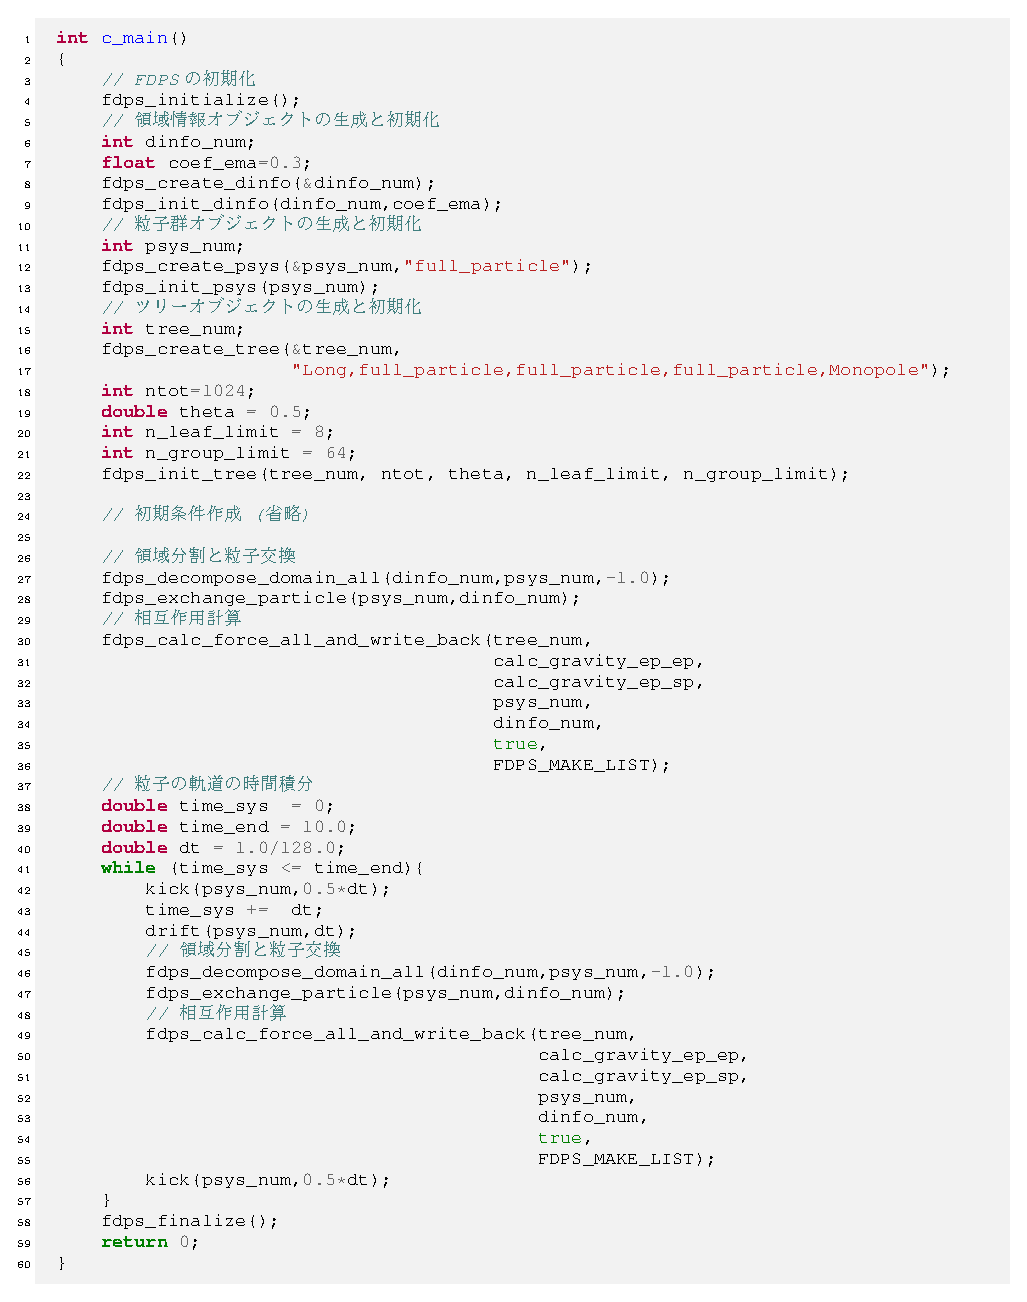
\includegraphics[width=8cm]{./fig/src_main_in_c.eps}
\caption{C言語でのメイン関数の実装例.関数\texttt{drift}, \texttt{kick}は,それぞれ粒子の位置と速度を時間積分する関数である.また,関数\texttt{calc\_gravity\_ep\_ep}, \texttt{calc\_gravity\_ep\_sp}はそれぞれ粒子間相互作用,粒子-超粒子間相互作用を計算する関数である.}
\label{fig:src_main_in_c}
\end{figure}


以上,C言語インターフェースの利用例についての簡単な説明を行った.Fortranインターフェースを用いる場合でも,メイン関数の構造はほぼ同じ構造となる.Fortranインターフェースを使った例に関しては,FDPSに付属するドキュメントや\cite{2018PASJ...70...70N}を参照されたい.


\section{まとめ}

我々はFDPS Ver.1をリリース以降今までに4回のメジャーアップデートを行っ
てきた.Ver.2およびVer.4では主にアクセラレータを搭載した計算機向けの機
能強化を行ってきた.結果,これらの追加機能を用いることでGPUを用いた計
算はCPUのみを用いた計算に比べて計算時間が10倍程度短くできることが分かっ
た.また,GyoukouやTaihuLight等の大規模ヘテロジニアスメニコアシステム
でも性能測定を行い非常に高い実行効率を達成することができた.

また,Ver.3およびVer.5ではFDPSをFortranやC言語から呼び出すためのインター
フェースの開発を行った.これらのインターフェースはFortranやC言語から
FDPSの機能を呼び出すためのAPIや,これらの言語で書かれた粒子データから
C++のクラスを生成するコードジェネレータを備えている.これらのインター
フェースを用いることでC++になじみの薄いFortranやC言語のユーザーも容易
にFDPSを使うことができる.

\begin{acknowledgment}

この研究は「次世代領域研究開発」(高性能汎用計算機高度利用補助金)「ヘ
  テロジニアス・メニーコア計算機による大規模計算科学」,計算科学振興財
団 研究教育拠点(COE)形成推進事業「 ポスト「京」,ポスト・ポスト「京」
  をみすえたハードウェア・アルゴリズム・ソフトウェアの総合的研究 」,
およびJSPS科研費(JP18K11334)の補助を受けています.

\end{acknowledgment}

%\bibliography{ms}

\begin{thebibliography}{9}

\bibitem{2014GROMACS}
Abrahama,~M.~J., Murtolad,~T., Schulzb,~R., Palla,~S., Smithb,~J., Hessa,~B. \& Lindahl.,~E.\ 2015, SoftwareX, 1, 19

\bibitem{1990JCoPh..87..161B} Barnes, J.~E.\ 1990, Journal of Computational Physics, 87, 161 

\bibitem{Bedorf:2014:PGT:2683593.2683600} B{\'e}dorf, J., Gaburov, E.,
  Fujii, M.~S., Nitadori, K., Ishiyama, T. and Zwart, S.~P.,
  Proceedings of the International Conference for High Performance
  Computing, Networking, Storage and Analysis, SC '14, Piscataway, NJ,
  USA, IEEE Press, pp.\ 54--65
  
\bibitem{fu2016sunway} Fu H, Liao J, Yang J, Wang L, Song Z, Huang X,
  Yang C, Xue W, Liu F, Qiao F et~al. 2016,  Science China Information Sciences, 59(7): 072001.

\bibitem{Hamada:2009:THN:1654059.1654123}
  Hamada,~T., Narumi,~T., Yokota,~R., Yasuoka,~K., Nitadori,~K., \& Taiji,~M.\ 2009, Proceedings of the Conference on High Performance Computing Networking, Storage and Analysis, 62, 1

\bibitem{2009PASJ...61.1319I} Ishiyama, T., Fukushige, T., \& Makino, J.\ 2009, \pasj, 61, 1319
  
\bibitem{2016PASJ...68...54I} Iwasawa, M., Tanikawa, A., Hosono, N., et al.\ 2016, \pasj, 68, 54

\bibitem{2018ICCS} Iwasawa, M., Long, W., Keigo, N., et al.\ 2018, Lecture Notes in Computer Science, vol 10860. Springer, Cham

\bibitem{2004PASJ...56..521M} Makino, J.\ 2004, \pasj, 56, 521
  
\bibitem{2018PASJ...70...70N} Namekata, D., Iwasawa, M., Nitadori, K., et al.\ 2018, \pasj, 70, 70 

\bibitem{1995LAMMPS} Plimpton,~S.\ 1995, J. Comp. Phys., 117, 1
  
\bibitem{2005MNRAS.364.1105S} Springel, V.\ 2005, \mnras, 364, 1105

\end{thebibliography}

\end{document}
